%! Author = trevo
%! Date = 2/22/2025

% Preamble
\documentclass[12pt]{report}
\usepackage{amsmath,setspace, enumerate,pdfpages,mathrsfs,hyperref,csquotes,graphicx,amsfonts,pdfpages}
\usepackage[british]{babel}


\usepackage[left=4cm, right=2cm, top=2cm, bottom=2cm, footskip=1cm]{geometry}




\usepackage[round]{natbib}
\bibliographystyle{plainnat}
\doublespacing
\setlength\parindent{24pt}
\setcounter{tocdepth}{3}






\begin{document}

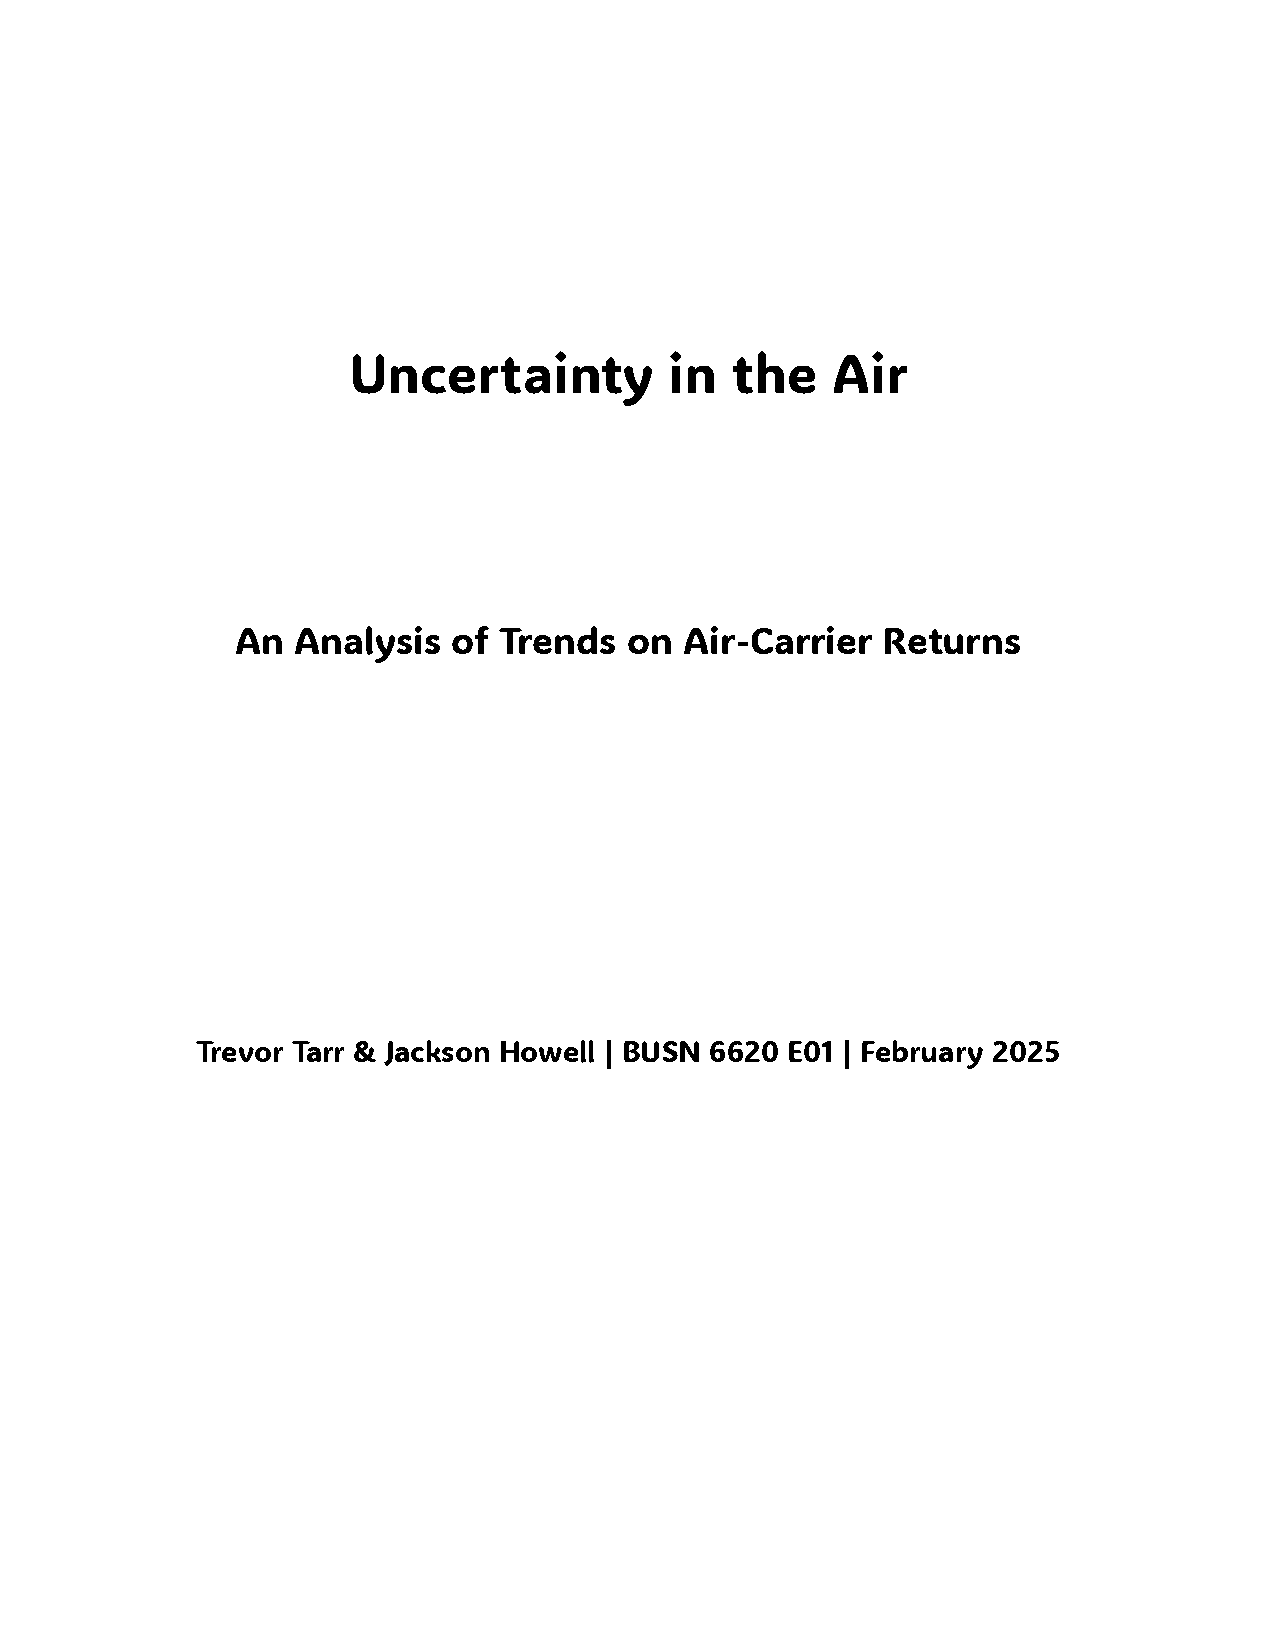
\includepdf{FFPFP}
    \newpage
\pagenumbering{gobble}
    \newpage
    \pagenumbering{roman}


\newpage
\tableofcontents
\newpage

\pagenumbering{arabic}
\chapter*{Abstract \& Hypothesis}
\addcontentsline{toc}{chapter}{Abstract \& Hypothesis}
\section*{\underline{Abstract}}
\addcontentsline{toc}{section}{Abstract}
With recent COVID-19, past terrorist attacks including 9/11, Boeing and Airbus planes successes and difficulties (like the Boeing MAX8), and various strikes both in the past and gearing up(future possible strikes [none known of as of 2/24/2025]) the team wanted to know how the bottom lines of airlines are impacted by these factors.
The team also wanted to take into account different airline models and strategies (low-cost and legacy) as each cater to different audiences when it comes to differences in offerings.
Low-cost carriers cater to the money-tight audiences and family travel while legacy prioritize comfort in travel, luxury travel, and business travel.
There are also differences in fleets and flight routes (domestic v.s. international) so factors like those also raised questions within the team.
\newpage
\section*{\underline{Hypothesis}}
The following hypothesises reflect how each trend effect the dependent variable defined as the percent change in monthly closing price of an airline's stock).

\addcontentsline{toc}{section}{Hypothesis}
\begin{enumerate}
    \item[Travel Restrictions:]: The implementation of travel restrictions generally correlates with declining airline stock prices, with larger fleet operators potentially experiencing a greater impact due to the broader scope of their operations affected.
    \item[Boeing Planes]: Negative views on a company who is associated with production of commercial air-crafts create uneasy sentiment especially for and towards airlines who fleet mainly comprise or include this manufactures air-crafts. This would lead to less travel on those airline lessening stock performace positive changes.
    \item[Airbus Planes]: A main competitor of Boeing. A similar hypothesis is in place for this variable as that of Boeing Planes.
    \item[Pilot Strikes]: Increased media coverage of pilot strikes often results in decreased investor confidence and lower airline stock prices due to fears of flight disruptions and reduced capacity brining down profits and stock performance.
    \item[Terrorism]: Heightened concern about terrorism, indicated by increased search interest, typically leads to lower airline stock prices, especially for international carriers, as passenger safety anxieties reduce travel demand brining down airline stock performance.


\end{enumerate}
\nocite{*}


\chapter*{Methodology}
\addcontentsline{toc}{chapter}{Methodology}



This research project investigates the influence of consumer
sentiment, as measured by search interest, on airline stock prices. The
following methodology was employed to analyze this relationship:

\section*{\underline{Variables}}
\addcontentsline{toc}{section}{Variables}
\begin{enumerate}
 \item[\underline{Independent}]: Trend Data (Google Trend Data).
   \addcontentsline{toc}{subsection}{Independent}
    These trend topics are to encapsulate various issues, risks, and interests theorized to impact the airline market.
        \begin{enumerate}
            \item[Travel Restriction]: This topic was chosen to highlight the news and trends on when travel is disrupted due to political or physical barriers to travel.
            This includes during pandemics, political instability, economic instability, infrastructure changes, or other factor disrupting travel.
            \item[Boeing Plane]: Boeing is one of the main manufacturers of commercial aircraft.
            This topic was chosen to highlight news on a supply line of an air-carrier.
            \item[Airbus Plane]: Airbus is the main competitor of Boeing in regard to the commercial aircraft manufacturing market.
            This topic was chosen to highlight and compare to Boeing Plane Trends.
            \item[Pilot Strike]: Pilots are the main employment positions for an air-carrier organization.
            This topic was chosen to highlight disruptions in the labour market category for air-carrier organizations.
            \item[Terrorism]: Terrorist acts create a sense of fear in customers to travel.
            This topic was chosen to highlight the travel demand with the news of fear and the threat of physical danger whether at home or abroad.
        \end{enumerate}
{\tiny Note: Singular forms were chosen over plural to account for seperated events involving planes, strikes, and restrictions.}


  \addcontentsline{toc}{subsection}{Dependent}
    \item[\underline{Dependent}]: Airline Closing Monthly Stock Prices.
    The airlines chosen are a sample from both Legacy and Low-Cost carriers as to observe trend data on both sectors within the industry.
    \begin{enumerate}
        \item[Legacy]: Airlines flying prior to airline deregulation in the 1970s and typically seen as luxury brands.
            \begin{enumerate}
                \item[1.]Delta Air Lines, Inc. (DAL)
                \item[2.]United Airlines Holdings, Inc. (UAL)
            \end{enumerate}
        \item[Low-Cost]: Airlines who focus on providing the basic flight packages rather than luxury travel.This lowers the costs of flying for customers but at the cut of luxuries that may include: full meal options, broad entertainment options, seat classes, etc. .
            \begin{enumerate}
                \item[3.]Southwest Airlines Co. (LUV)
                \item[4.]Allegiant Travel Company (ALGT)
            \end{enumerate}
    \end{enumerate}


\end{enumerate}

\section*{\underline{Data Collection}}
\addcontentsline{toc}{section}{Data Collection}


\subsection*{Dependent Variables}
Data collection for Dependent Variables was gathered from Historical Data from Yahoo Finance using tickers: UAL, DAL, LUV, ALGT. This data was then transferred to a Microsoft Excel notebook.


Subsequently, the percentage change
in the monthly closing stock price was calculated for each airline to
facilitate the analysis.





\\ \\
\subsection*{Independent Variables}
Data collection for Independent variables were gathered from worldwide monthly Google Trend data values over the maximum amount stored by Google Trends (2004 onwards).

Google Trends provides normalized search interest data, where a value of
100 represents the peak popularity for a given search term during the specified
time period.


This data was downloaded as a .csv file and opened and used in a separate Microsoft Excel sheet in the same notebook as the Dependent variable data.


\section*{\underline{Analysis Methodology}}
\addcontentsline{toc}{section}{Analysis Methodology}
\subsection*{Data Processing}
\addcontentsline{toc}{subsection}{Data Processing}


All collected data, including both search interest and stock
price data, was organized into a time series format. The time range for the
independent variables, or the search interests, and the dependent variables,
the stock price changes, was maintained consistently for each airline to ensure
model accuracy

\par


The percent change in closing price was calculated for each airline
to normalize the data and facilitate comparison between different airlines.
This transformation allows for a standardized comparison of the relative
fluctuations in stock prices, regardless of their value.


\subsection*{Regression Analysis}
\addcontentsline{toc}{subsection}{Regression Analysis}


A multiple linear regression model was employed to quantify
the relationship between consumer sentiment, as proxied by search interest, and
airline stock price changes. The following regression equation was specified
for each airline:


\[ \text{Stcok Price Change} =   r\text{(TRI)} + n\text{(BPI) }+\\ a\text{(API)} + p\text{(PSI)} + t\text{(TSI)} + b + \epsilon\]

Where:
\begin{enumerate}
    \item $r, n,a, p, \& t $ are the coefficients for each respective search interest variable, representing their impact on the airline's stock price change.
    \item $b$ is the intercept.
    \item $\epsilon$ is the error term, capturing the unexplained variance in stock price changes.
    \item TRI: Travel Restrictions Search Interest.
    \item BPI:Boeing Planes Search Interest.
    \item API:Airbus Planes Search Interest.
    \item PSI:Pilot Strike Search Interest.
    \item TSI:Terrorism Search Interest.

\end{enumerate}

\subsection*{Statistical Significance}
\addcontentsline{toc}{subsection}{Statistical Significance}


The statistical significance of each independent variable
was assessed using t-statistics and associated p-values. A significance level
of $t\geq 2$ was used to determine whether a predictor variable had a
statistically significant relationship with the airline's stock price change. The $p$ value was used to check whether to accept or reject the null hypothesises (our hypothesises) with a value below $.05$ having us reject the hypothesis and at or above accepting.


\subsection*{Model Fitness}
\addcontentsline{toc}{subsection}{Model Fitness}
The fitness of a model with respected data was scored using $R^2$ value ($r2$). As the score gets closer to $1$ the model better fits the data with a lower limit of 0.
\subsection*{Interpretation}
\addcontentsline{toc}{subsection}{Interpretation}
Estimated coefficients (r,n,a,p,and t) used in the models are interpreted to understand impact of each search terms interest on each airline's stock price change monthly.

\newpage
\chapter*{Results and Interpertations}
\addcontentsline{toc}{chapter}{Results and Interpertations}
The following section is the collection of results and brief industry related discussions gathered from the analysis of the trends against the airline percent change in closing stock value for United, Delta, Southwest, Allegiant.
\section*{\underline{United}}
\addcontentsline{toc}{section}{United}
\subsection*{Results:}

\begin{enumerate}

 \setlength{\itemsep}{1.5cm}

    \item[\underline{Travel Restriction:}]
        \begin{enumerate}
            \item[$R^2$]:0.0014564929850374
            \item[]
                \begin{tabular}{|c|c|c|c|}
                          \toprule \hline
                          \textbf{Variable} & \textbf{Coefficients} & \textbf{t Stat} & \textbf{P-Val.}\\ \hline
                          Intercept & 0.020181 & 1.70072 &.0903 \\ \hline
                          Travel restrictions:(Worldwide) & -0.0003 & -0.57415 &.5664 \\ \hline
                          \bottomrule





                \end{tabular}




        \end{enumerate}

    \item[\underline{Boeing Plane:}]
        \begin{enumerate}
            \item[$R^2$]:0.000260007235396399
            \item[]
                 \begin{tabular}{|c|c|c|c|}

        \toprule \hline
        \textbf{Variables} & \textbf{Coefficients}  & \textbf{t Stat}& \textbf{P-Val.} \\ \hline

        Intercept & 0.021248 &  1.107273 &.2693 \\ \hline
        Boeing Planes: (Worldwide) & -0.00027 &  -0.24244 &.808659\\ \hline
        \bottomrule

                \end{tabular}




        \end{enumerate}

    \item[\underline{Airbus Plane:}]
 \begin{samepage}

        \begin{enumerate}
            \item[$R^2$]:0.00266981946070099
            \item[]
                \begin{tabular}{|c|c|c|c|}

                \toprule \hline
                \textbf{Variables} & \textbf{Coefficients}  & \textbf{t Stat}& \textbf{P-Val.} \\ \hline

                Intercept & 0.041836 &  1.259387 &.20919 \\ \hline
                Airbus Planes: (Worldwide) & -0.00072 &  -0.77781&.437492 & \\ \hline
                \bottomrule
                \end{tabular}

        \end{enumerate}
\end{samepage}
    \item[\underline{Pilot Strike:}]
 \begin{samepage}


        \begin{enumerate}
            \item[$R^2$]:0.00000855554529986246
            \item[]
                \begin{tabular}{|c|c|c|c|}



        \toprule \hline
        \textbf{Variables} & \textbf{Coefficients}  & \textbf{t Stat} & \textbf{P-Val.}\\ \hline

        Intercept & 0.017719081 &  1.371277& .171649 \\ \hline
        Pilot Strike: (Worldwide) & -4.08225E-05  & -0.04397 &.964965 \\ \hline
        \bottomrule

                \end{tabular}

        \end{enumerate}
\end{samepage}

    \item[\underline{Terrorism:}]
        \begin{enumerate}
            \item[$R^2$]:0.00240540054576054
        \item[$$]\begin{tabular}{|c|c|c|c|}



        \toprule \hline
        \textbf{Variables} & \textbf{Coefficients}  & \textbf{t Stat}& \textbf{P-Val.} \\ \hline

        Intercept & 0.037468 &  1.280877 &.20155\\ \hline
        Terrorism: (Worldwide) & -0.00099 & -0.73819 &.461162 \\ \hline
        \bottomrule



                \end{tabular}

    \end{enumerate}
    \item[\underline{All:}]
 \begin{samepage}



    \begin{enumerate}
        \item[$R^2$]:0.0133217114539175
        \item[]\begin{tabular}{|c|c|c|c|}
        \toprule \hline
        \textbf{Variables} & \textbf{Coefficients} & \textbf{t Stat}& \textbf{P-Val.} \\ \hline

        Intercept & 0.103013282 &  1.955146 &.051821 \\ \hline
        Travel restrictions: (Worldwide) & -0.000739918 & 0 -1.24247 & .215375\\ \hline
        Boeing Plane: (Worldwide) & 0.001231399 &  0.688808 &.491663 \\ \hline
        Airbus Plane: (Worldwide) & -0.001957029 &  -1.2429 &.215215 \\ \hline
        Pilot Strike: (Worldwide) & 0.000129146 &  0.136284 & .89172 \\ \hline
        Terrorism: (Worldwide) & -0.001531551 &  -1.07378 & .284088\\ \hline
        \bottomrule
    \end{tabular}









    \end{enumerate}
\end{samepage}
\end{enumerate}
\subsection*{Interpretation:}



The analysis of United Airlines revealed a positive
correlation between its stock price and search interest in Boeing
Plane and Pilot Strike. The positive relationship with
Boeing Plane may suggest that searches related to Boeing aircraft
are associated with positive developments and United, such as new deals or
orders, rather than negative events like plane failures.
It is also possible that pilot strikes, while impactful, occur less frequently or have a
comparatively smaller effect on United's operations than on other airlines.
Conversely, a negative relationship was observed between United's stock price
and searches for Travel Restriction, Airbus Plane,
and Terrorism. The negative impact of Travel
Restriction is consistent with the general understanding that such
restrictions negatively affect the entire airline industry.
While United's fleet does not include Airbus aircraft, negative news or sentiment surrounding
Airbus may still affect overall market sentiment and thus impact United's stock
price.
As expected, increased searches related to Terrorism correlate with a decrease in United's stock price, reflecting the negative impact of security concerns on air travel demand.





\newpage
\section*{\underline{Delta}}
\addcontentsline{toc}{section}{Delta}
\subsection*{Results:}
\begin{enumerate}
    \item[\underline{Travel Restriction:}]
        \begin{enumerate}
            \item[$R^2$]:0.000974704742830236
            \item[]:


                \begin{tabular}{|c|c|c|}
                    \toprule\hline
                    \textbf{Variables} & \textbf{Coefficients} & \textbf{t Stat}& \textbf{P-Val.} \\ \hline
                    Intercept & 0.015285 & 1.603178&.11039 \\ \hline
                    Travel restriction:(Worldwide) & -0.00019 & -0.45372 &.650495\\ \hline
                    \bottomrule
                \end{tabular}





        \end{enumerate}
    \item[\underline{Boeing Plane:}]
        \begin{enumerate}
            \item[$R^2$]:0.000871425842435283
            \item[]:

                \begin{tabular}{|c|c|c|c|}
                    \toprule \hline

                    \textbf{Variables} & \textbf{Coefficients} & \textbf{t Stat}& \textbf{P-Val.} \\ \hline

                    Intercept & 0.008284 & 0.553962 &.580191 \\ \hline
                    Boeing Plane: (Worldwide) & 0.000368 & 0.428989 &.668369  \\ \hline
                    \bottomrule
                \end{tabular}





        \end{enumerate}
    \item[\underline{Airbus Plane:}]
        \begin{enumerate}
            \item[$R^2$]:0.0000744087250069324
            \item[]:


                \begin{tabular}{|c|c|c|c|}
                    \toprule \hline
                    \textbf{Variables} & \textbf{Coefficients} & \textbf{t Stat} & \textbf{P-Val.}\\ \hline

                    Intercept & 0.01658 & 0.636965 &.524838 \\ \hline
                    Airbus Plane: (Worldwide) & -9.2E-05 & -0.12531 &.900401 \\ \hline
                    \bottomrule
                \end{tabular}




        \end{enumerate}
    \item[\underline{Pilot Strike:}]
        \begin{enumerate}
            \item[$R^2$]:0.00254097586946747
            \item[]:


                \begin{tabular}{|c|c|c|c|}
                    \toprule \hline
                    \textbf{Variable} & \textbf{Coefficients} & \textbf{t Stat}& \textbf{P-Val.} \\ \hline

                    Intercept & 0.018552 & 1.674289& .095555\\ \hline
                    Pilot Strike: (Worldwide) & -0.00072 & -0.73315 &.46428 \\ \hline
                    \bottomrule
                \end{tabular}





        \end{enumerate}
    \item[\underline{Terrorism:}]
        \begin{enumerate}
            \item[$R^2$]:
            \item[]:

                \begin{tabular}{|c|c|c|c|}
                    \toprule \hline
                    \textbf{Variables} & \textbf{Coefficients} & \textbf{t Stat} &\textbf{P-Val.}\\ \hline

                    Intercept & 0.031217 & 1.170699& .24304\\ \hline
                    Terrorism: (Worldwide) & -0.00093 & -0.70251 &.483133 \\ \hline
                    \bottomrule
                \end{tabular}





        \end{enumerate}
    \item[\underline{All:}]
        \begin{enumerate}
            \item[$R^2$]:0.0141519669709025
            \item[]:


                \begin{tabular}{|c|c|c|c|}
                    \toprule \hline
                    \textbf{Variables} & \textbf{Coefficients} & \textbf{t Stat} &\textbf{P-Val.}\\ \hline

                    Intercept & 0.080801 & 1.645365&.101412 \\ \hline
                    Travel restriction: (Worldwide) & -0.00054 & -1.11771 &.264984 \\ \hline
                    Boeing Plane: (Worldwide) & 0.001224 & 0.871276& .384613 \\ \hline
                    Airbus Plane: (Worldwide) & -0.00122 & -0.9624 &.336972 \\ \hline
                    Pilot Strike: (Worldwide) & -0.0009 & -0.88212 &.378737 \\ \hline
                    Terrorism: (Worldwide) & -0.0017 & -1.15071&.251181 \\ \hline
                    \bottomrule
                \end{tabular}





        \end{enumerate}
\end{enumerate}
\subsection*{Interpretation:}
We see a positive coefficient between returns and Boeing planes which shows that ultimately there have been a positive impact of Boeing on delta returns.
This could be from newer planes and FAA clearances on planes used by Delta having a positive impact in the travel consumer market.
This supports the $.26$ P-value and 1.2 t-Stat. and thus having a stronger relationship.
Travel Restrictions, Pilot Strikes, Terrorism and Airbus all have negative coefficients (Airbus' though very slightly negative)
aligns with predictions as Delta has a mix of Airbus and Boeing planes (with the Boeing slightly more positive may indicate slightly more reliance on Boeing Planes in the among trends)
and thought son Travel Restrictions, Pilot Strikes and Terrorism (supported by higher t-stat values and P-Values).
\newpage
\section*{\underline{Southwest}}
\addcontentsline{toc}{section}{Southwest}
\subsection*{Results:}
\begin{enumerate}
    \item[\underline{Travel Restriction:}]
        \begin{enumerate}
            \item[$R^2$]:0.000817955370534399
            \item[]:

                \begin{tabular}{|c|c|c|c|}
                    \toprule\hline
                    \textbf{Variables} & \textbf{Coefficients} & \textbf{t Stat} &\textbf{P-Val.} \\\hline

                    Intercept & 0.008044 & 1.280276 &.2 \\\hline
                    Travel restriction:(Worldwide) & -0.00013 & -0.45329 &.065\\\hline
                    \bottomrule
                \end{tabular}




        \end{enumerate}
    \item[\underline{Boeing Plane:}]
        \begin{enumerate}
            \item[$R^2$]:0.00504137252033226
            \item[]:

                \begin{tabular}{|c|c|c|c|}
                    \toprule\hline
                    \textbf{Variable} & \textbf{Coefficients} & \textbf{t Stat}&\textbf{P-Val.} \\ \hline

                    Intercept & 0.017032 & 1.598372 &.1112 \\ \hline
                    Boeing Plane: (Worldwide) & -0.00066 & -1.12774 & .26\\ \hline
                    \bottomrule
                \end{tabular}




        \end{enumerate}
    \item[\underline{Airbus Plane:}]
        \begin{enumerate}
            \item[$R^2$]:0.00750791874428054
            \item[]:
                \begin{tabular}{|c|c|c|c|}
                    \toprule\hline
                    \textbf{Variable} & \textbf{Coefficients} & \textbf{t Stat}&\textbf{P-Val.} \\\hline

                    Intercept & 0.027304 & 1.72049 & .086576\\ \hline
                    Airbus Plane: (Worldwide) & -0.00059 & -1.37795 & .169\\ \hline
                    \bottomrule
                \end{tabular}




        \end{enumerate}
    \item[\underline{Pilot Strike:}]
        \begin{enumerate}
            \item[$R^2$]:0.00216618830881419
            \item[]:


                \begin{tabular}{|c|c|c|c|}
                    \toprule \hline
                    \textbf{Variable} & \textbf{Coefficients} & \textbf{t Stat} &\textbf{P-Val.}\\ \hline

                    Intercept & 0.009599 & 1.408238 &.16029\\ \hline
                    Pilot Strike: (Worldwide) & -0.00036 & -0.73817 &.461101\\ \hline
                    \bottomrule
                \end{tabular}



        \end{enumerate}
    \item[\underline{Terrorism:}]
        \begin{enumerate}
            \item[$R^2$]:0.000775486385304982
            \item[]:


                \begin{tabular}{|c|c|c|c|}
                    \toprule \hline
                    \textbf{Variables} & \textbf{Coefficients} & \textbf{t Stat} &\textbf{P-Val.}\\ \hline

                    Intercept & 0.010975 & 1.012495 &.3122\\ \hline
                    Terrorism: (Worldwide) & -0.00017 & -0.44136&.659333 \\ \hline
                    \bottomrule
                \end{tabular}




        \end{enumerate}
    \item[\underline{All:}]
        \begin{enumerate}
            \item[$R^2$]:0.0140397082194081
            \item[]


                \begin{tabular}{|c|c|c|c|}
                    \toprule \hline
                    \textbf{Variables} & \textbf{Coefficients} & \textbf{t Stat}&\textbf{P-Val.} \\ \hline

                    Intercept & 0.041824 & 1.967885 &.0502 \\ \hline
                    Travel restriction: (Worldwide) & -0.00033 & -1.03686 &.0502 \\ \hline
                    Boeing Plane: (Worldwide) & -0.00012 & -0.15461 &.300815 \\ \hline
                    Airbus Plane: (Worldwide) & -0.00063 & -1.05257&.8772 \\ \hline
                    Pilot Strike: (Worldwide) & -0.00031 & -0.63867&.293566 \\ \hline
                    Terrorism: (Worldwide) & -0.00026 & -0.63055&.528918 \\ \hline
                    \bottomrule
                \end{tabular}



        \end{enumerate}
\end{enumerate}
\subsection*{Interpretation:}
The slight negative relationship between Travel Restrictions and Southwest flight makes sense as since Southwest is primarily a domestic carrier and travel restrictions mainly effect international travel show that any travel restriction have minor negative impact on Southwest's performance.
With a slightly negative coefficient and using the associated p-value we can accept our hypothesis that there is some effect on Southwests return performance when it comes to Boeing news.
This can be due to consumers not wanting to fly on a Boeing plane when news of crashes and issues arise but also with flagship planes consumers may be slightly eager to fly on the newest models.
Regarding Airbus Plane trends, similarly to Boeing (with $R^2$, t-Stat and P value) we can accept the hypothesis. The smaller relationship was expected as since Southwest does not operate Airbus planes.
The small relationship may come from those looking after Boeing incidents to see if Southwest may decide to add some to its fleet.
The negative relationship with Pilot Strike is expected and confirms our hypothesis (p-value) as any disruptions in the labour force will in turn affect the business of Southwest. With a t-Stat of $1.4$ there is some statistical significance.
Finally, the negative relationship with Terrorism is expected and confirmed (p-value, and t-stat as somewhat significant statistically) as when fear is introduced into the marketplace, consumers may refuse to travel at a higher rate lessening demand in air travel.
The "All" analysis was conducted to see simultaneous effect and reflects what was talked about above.

\newpage
\section*{\underline{Allegiant}}
\addcontentsline{toc}{section}{Allegiant}
\subsection*{Results:}
\begin{enumerate}
    \item[\underline{Travel Restriction:}]
        \begin{enumerate}
            \item[$R^2$]: 0.000158409806922983
            \item[]
                \begin{tabular}{|c|c|c|c|}
                    \toprule \hline
                    \textbf{} & \textbf{Coefficients}  & \textbf{t Stat}&\textbf{P-Val.} \\ \hline

                    Intercept & 0.013366 &  1.444341 & .150092\\ \hline
                    Travel restrictions:(Worldwide) & -7.4E-05 &  -0.18499 &.853409 \\ \hline
                    \bottomrule
                \end{tabular}





        \end{enumerate}
    \item[\underline{Boeing Plane:}]
        \begin{enumerate}
            \item[$R^2$]:0.00229054632984585
            \item[]

                \begin{tabular}{|c|c|c|c|}
                    \toprule \hline
                    \textbf{Variables} & \textbf{Coefficients}  & \textbf{t Stat}&\textbf{P-Val.} \\ \hline
                    Intercept &0.0210912936852673 &  1.44078 &.151095 \\ \hline
                    Boeing Plane: (Worldwide) & -0.00059  & -0.7042 &.482068 \\ \hline
                    \bottomrule
                \end{tabular}




        \end{enumerate}
    \item[\underline{Airbus Plane:}]
        \begin{enumerate}
            \item[$R^2$]:0.00419036191845844
            \item[]

            \begin{tabular}{|c|c|c|c|}
                    \toprule  \hline
                    \textbf{Variables} & \textbf{Coefficients} &  \textbf{t Stat}&\textbf{P-Val.} \\  \hline

                    Intercept & 0.03558 &  1.396969 &.163856\\  \hline
                    Airbus Plane: (Worldwide) & -0.00068 & -0.95338 &.341465 \\  \hline
                    \bottomrule
                \end{tabular}

        \end{enumerate}
    \item[\underline{Pilot Strike:}]
        \begin{enumerate}
            \item[$R^2$]:0.00453590804961368
            \item[]

                \begin{tabular}{|c|c|c|c|}
                    \toprule  \hline
                    \textbf{Variables} & \textbf{Coefficients}   & \textbf{t Stat}&\textbf{P-Val.} \\  \hline

                    Intercept & 0.019231  & 1.795156 &.074027 \\  \hline
                    Pilot Strike: (Worldwide) & -0.00096  & -0.99208 &.322269 \\  \hline
                    \bottomrule
                \end{tabular}





        \end{enumerate}
    \item[\underline{Terrorism:}]\\
        \begin{enumerate}
            \item[$R^2$]:0.000000563450974027640
            \item[]


                \begin{tabular}{|c|c|c|c|}
                    \toprule  \hline
                    \textbf{Variables} & \textbf{Coefficients} & \textbf{t Stat}&\textbf{P-Val.} \\  \hline

                    Intercept & 0.012400357 &  0.487219 &.626597 \\  \hline
                    Terrorism: (Worldwide) & 1.36349E-05 & 0.011032 & .9912\\  \hline
                    \bottomrule
                \end{tabular}





        \end{enumerate}
    \item[\underline{All:}]
    \begin{samepage}

        \begin{enumerate}
            \item[$R^2$]:0.0102953329441835
            \item[]
                \begin{tabular}{|c|c|c|c|}
                    \toprule  \hline
                    \textbf{Variables} & \textbf{Coefficients} & \textbf{t Stat}&\textbf{P-Val.} \\  \hline

                    Intercept & 0.062231 &  1.345729 & .179827\\  \hline
                    Travel restriction: (Worldwide) & -0.00034 &  -0.71564 & .475003\\  \hline
                    Boeing Plane: (Worldwide) & 8.42E-05 &  0.061342 &.951144\\  \hline
                    Airbus Plane: (Worldwide) & -0.00085 &  -0.69962 &.48493 \\  \hline
                    Pilot Strike: (Worldwide) & -0.00099 &  -0.98374 &.326366 \\  \hline
                    Terrorism: (Worldwide) & -0.00062 &  -0.4527 &.651229 \\  \hline
                    \bottomrule
                \end{tabular}





        \end{enumerate}
        \end{samepage}
\end{enumerate}
\subsection*{Interpretation:}



For Allegiant, a positive relationship was found between its
stock price and searches for Boeing Planes, although the magnitude
of this relationship was relatively low. This is likely due to the fact that
Allegiant's fleet does not include any Boeing aircraft. Similar to other airlines, Allegiant's stock
price showed a negative relationship with searches for Travel
Restrictions, Airbus Planes, Pilot Strikes, and
Terrorism. The negative impact of Travel Restrictions
is consistent across the industry. Since Allegiant exclusively operates Airbus aircraft, negative news or sentiment
related to Airbus planes could have a more pronounced effect on their stock
price. As with other airlines, increased
searches related to Terrorism relate with decreased stock
prices, reflecting the negative impact on travel demand.
However, since Allegiant only operates domestic flights, the negative impacts are lessened to domestic related or air-travel matters.





\newpage







\chapter*{Conclusion, Recommendations, \& Bibliography}
\addcontentsline{toc}{chapter}{Conclusion, Recommendations \& Bibliography}
\section*{Conclusion}
\addcontentsline{toc}{section}{Conclusion}
Overall, the models regressed have some significance.
While some models have higher significance then others, the overall sentiment is that these trends do have a major impact (together or apart)
on an air-carriers bottom line. Increased search activity related one manufacturer fleets resulted in a more significant change in the airline's stock from search trends on the specific manufacturer.
price alone. The impact of Terrorism and Travel Restriction searches were
less for Southwest and Allegiant compared to United and Delta, potentially
reflect Southwest's and Allegiances primarily domestic operations with limited international
exposure from Southwest. Restricting travel through either government policy or through other barriers acts in a similar fashion forcing customers to rethink travel plans. On average, searches related to Airbus Planes had the largest impact on decreasing stock prices across the airlines.
Finally, on average, searches related to Boeing Planes had the largest positive impact on stock prices.



\section*{Recommendations}
Based on the analysis conducted, several recommendations can be given to airline to mitigate risks and further optimize market returns:

Regarding Travel Restrictions, airlines should be aware of geopolitical sensitivities and  instability and optimize routes appropriately especially in high risk areas and during health emergencies.
Regarding air-craft manufacturers, airlines should understand current sentiment about public sentiment  regarding aircraft models and manufacturers and optimize routes accordingly.
Airlines should also leverage positive news and updates from the FAA that may show to positively reinforce public sentiment in travel.

While Pilot Strikes are of concern, our studies show they have minimal impact on returns.
This allows airlines to reallocate resources towards more impactful matters.
Finally, in regard to Terrorism, airlines should maintain heightened vigilance, and proactive approaches to ensuring the multi-factored approach to safety, security which play a vital role in the overall stock performance.
In line with the recommendations put forth regarding Travel restrictions, airlines should have fully operating and on-call ready emergency management and crisis divisions for contingency planing and execution at a moments notice.

\par
While this study provides a comprehensive analysis on the relationship between search trends and airline stock performance, further research could enhance the understanding and application of this data.
One such opportunity is with a correlation study that would focus on delving into specific relationship between the variables and airline returns change.
Such analysis would further allow for more in-depth data driven decisions and direction given when dealing with the variable that airlines face daily.

\addcontentsline{toc}{section}{Recommendations}
\newpage



    \bibliography{resources}
    \addcontentsline{toc}{section}{Bibliography}
\end{document}
